\documentclass[sigconf,nonacm]{acmart}

\usepackage{booktabs}
\usepackage{graphicx}
\usepackage{amsmath}
\usepackage{microtype}
\usepackage{balance}

\title{Evaluating Out-of-Core Analytical Execution: Buffer Pools vs. Memory-Mapped Streaming across the Parquet Row-Group Continuum}

\author{Nadeem Theba}
\affiliation{%
  \institution{Department of Computer Science \& Engineering}
  \city{Workstation Systems Lab}
  \country{USA}
}
\email{nadeemtheba@example.com}

\begin{abstract}
Analytical database engines increasingly process datasets exceeding physical main memory. Modern systems employ two dominant paradigms for memory-constrained analytical processing: explicit engine-managed buffer pools (e.g., DuckDB) and implicit memory-mapped OS streaming (e.g., Polars over \texttt{mmap}). However, the interaction between these execution architectures, underlying storage granularity (Parquet row-group sizes), and Linux kernel memory reclamation mechanics under severe cgroup constraints remains insufficiently quantified.

In this paper, we present an empirical evaluation of DuckDB (buffer pool manager) versus Polars (mmap streaming engine) operating under kernel-enforced memory throttling (\texttt{memory.high = 1G}) on a bare-metal Intel Core i5-10300H testbed with NVMe storage. We evaluate a 6-point Parquet row-group continuum ranging from 10K to 1M rows over TPC-H \texttt{lineitem} projections (>1.2GB uncompressed). Using high-frequency 20ms cgroups v2 telemetry and hardware PMU counters, we demonstrate that DuckDB's managed buffer pool maintains predictable query latency by explicitly evicting LRU blocks to NVMe scratch space. Conversely, Polars' \texttt{mmap} architecture suffers severe performance degradation at extreme row-group sizes due to kernel direct reclaim stalls (\texttt{allocstall}) and major page fault thrashing (\texttt{pgmajfault}). We identify 122K rows per row-group as the optimal out-of-core Pareto frontier boundary, offering up to $2.1\times$ lower latency than non-optimal configurations.
\end{abstract}

\begin{document}

\maketitle

\section{Introduction}
Analytical query processing engines are frequently deployed on resource-constrained hardware, edge devices, or shared cloud instances where available RAM is significantly smaller than dataset sizes. To handle out-of-core workloads without throwing Out-Of-Memory (OOM) fatal exceptions, analytical engines rely on two fundamental architectural approaches:
\begin{enumerate}
    \item \textbf{Engine-Managed Buffer Pools}: Systems such as DuckDB allocate a fixed-size memory buffer and implement custom eviction algorithms (e.g., LRU/2Q) to flush unpinned execution blocks directly to disk scratch storage.
    \item \textbf{Memory-Mapped OS Streaming}: Systems such as Polars map storage files directly into virtual memory via \texttt{mmap()} and delegate page cache eviction, prefetching, and page table swapping to the host operating system kernel.
\end{enumerate}

While Apache Parquet has become the de facto columnar storage format, file metadata configuration---specifically **Row-Group Granularity**---exerts a profound influence on I/O amplification and memory footprint. Small row groups reduce memory footprint per batch but increase metadata parsing overhead and file footer decompression churn. Large row groups maximize vectorization and compression efficiency but force large memory allocations during decompression, causing severe memory pressure under strict RAM limits.

\subsection{Contributions}
This paper makes the following key contributions:
\begin{itemize}
    \item \textbf{Controlled Experimental Sandbox}: We establish a fully reproducible 60-run interleaved benchmark suite under Linux cgroups v2 (\texttt{memory.high = 1G}, \texttt{memory.swap.max = 0}) on bare-metal NVMe hardware.
    \item \textbf{Parquet Row-Group Continuum Evaluation}: We systematically measure 6 row-group sizes ($10K, 50K, 122K, 250K, 500K, 1M$) across DuckDB and Polars.
    \item \textbf{Kernel-Level Telemetry}: Using 20ms cgroups v2 sampling, we quantify the exact cost of OS direct memory reclamation stalls (\texttt{allocstall}) and major page faults (\texttt{pgmajfault}).
    \item \textbf{Pareto Frontier Identification}: We establish that $122K$ rows per row-group represents the optimal Pareto trade-off between metadata overhead and page-fault thrashing.
\end{itemize}

\section{System Architecture \& Eviction Models}
The core distinction between DuckDB and Polars lies in their memory management and I/O execution contracts.

\subsection{DuckDB: Explicit Buffer Management}
DuckDB implements a dedicated Buffer Manager that regulates memory allocations across execution pipelines. When total query allocations approach the configured limit (\texttt{SET max\_memory = '1GB'}), the Buffer Manager selects unpinned data blocks and serializes them to a dedicated NVMe temp directory (\texttt{temp\_directory}).
The total execution cost model for DuckDB is expressed as:
\begin{equation}
T_{\text{DuckDB}} = T_{\text{scan}} + T_{\text{decompress}} + T_{\text{compute}} + N_{\text{spill}} \times (t_{\text{write\_NVMe}} + t_{\text{read\_NVMe}})
\end{equation}
Because DuckDB explicitly controls page eviction, it avoids kernel thread blocking and maintains deterministic query execution.

\subsection{Polars: Implicit OS Paging via \texttt{mmap}}
Polars utilizes Rust's Arrow implementation coupled with Rayon work-stealing parallelism. Columnar Parquet data is mapped into virtual address space via \texttt{mmap()}. When intermediate hash aggregation state exceeds cgroup memory limits, Polars does not spill to disk directly. Instead, the Linux kernel cgroups v2 memory controller catches allocation requests exceeding \texttt{memory.high = 1G} and forces the allocating thread into synchronous direct memory reclaim (\texttt{allocstall}).

The memory-mapped execution time model is governed by:
\begin{equation}
T_{\text{Polars}} = T_{\text{scan}} + T_{\text{compute}} + N_{\text{faults}} \times t_{\text{page\_fault}} + T_{\text{allocstall}}
\end{equation}
where $t_{\text{page\_fault}}$ represents the latency of a kernel page-fault interrupt (\#PF) requiring blocking NVMe random reads.

\section{Experimental Methodology}

\subsection{Hardware Testbed \& Isolation}
All benchmarks were executed on a dedicated bare-metal testbed:
\begin{itemize}
    \item \textbf{Processor}: Intel Core i5-10300H @ 2.50GHz (4 physical cores, 8 threads, 8MB L3 cache).
    \item \textbf{Memory}: 8GB DDR4-2933 MHz RAM.
    \item \textbf{Storage}: WDC PC SN730 512GB PCIe 3.0 x4 NVMe SSD formatted with \texttt{ext4}.
    \item \textbf{Operating System}: Ubuntu 24.04 LTS (Linux Kernel 6.8.0).
\end{itemize}

To isolate execution state, CPU affinity was locked to physical cores 0--3 via \texttt{taskset -c 0,1,2,3}. CPU scaling governors were set to \texttt{performance}. Prior to every trial, the Linux OS page cache was completely invalidated using:
\begin{verbatim}
sync && echo 3 > /proc/sys/vm/drop_caches
\end{verbatim}

\subsection{cgroups v2 Sandbox}
A dedicated Linux cgroup v2 node was provisioned at \texttt{/sys/fs/cgroup/benchmark} with:
\begin{itemize}
    \item \texttt{memory.high = 1073741824} (1.0 GB soft limit enforcing direct reclaim).
    \item \texttt{memory.max = 1610612736} (1.5 GB hard limit preventing instant OOM kills).
    \item \texttt{memory.swap.max = 0} (Disabled swap space to enforce true NVMe I/O paging).
\end{itemize}

\subsection{Workload \& Data Generator}
We synthesized a TPC-H SF10 \texttt{lineitem} dataset (60,000,000 records, ~1.2GB compressed Parquet). We generated 6 dataset variants by altering row-group boundary limits during export: $10K, 50K, 122K, 250K, 500K, 1M$.
The benchmark query executes a wide projection and high-cardinality aggregation:
\begin{verbatim}
SELECT l_orderkey % 500000 AS grp,
       COUNT(*) AS cnt,
       SUM(l_extendedprice) AS total_price,
       AVG(l_discount) AS avg_discount,
       SUM(l_quantity) AS total_qty
FROM lineitem
GROUP BY l_orderkey % 500000;
\end{verbatim}

\section{Empirical Evaluation}

\begin{figure}[t]
    \centering
    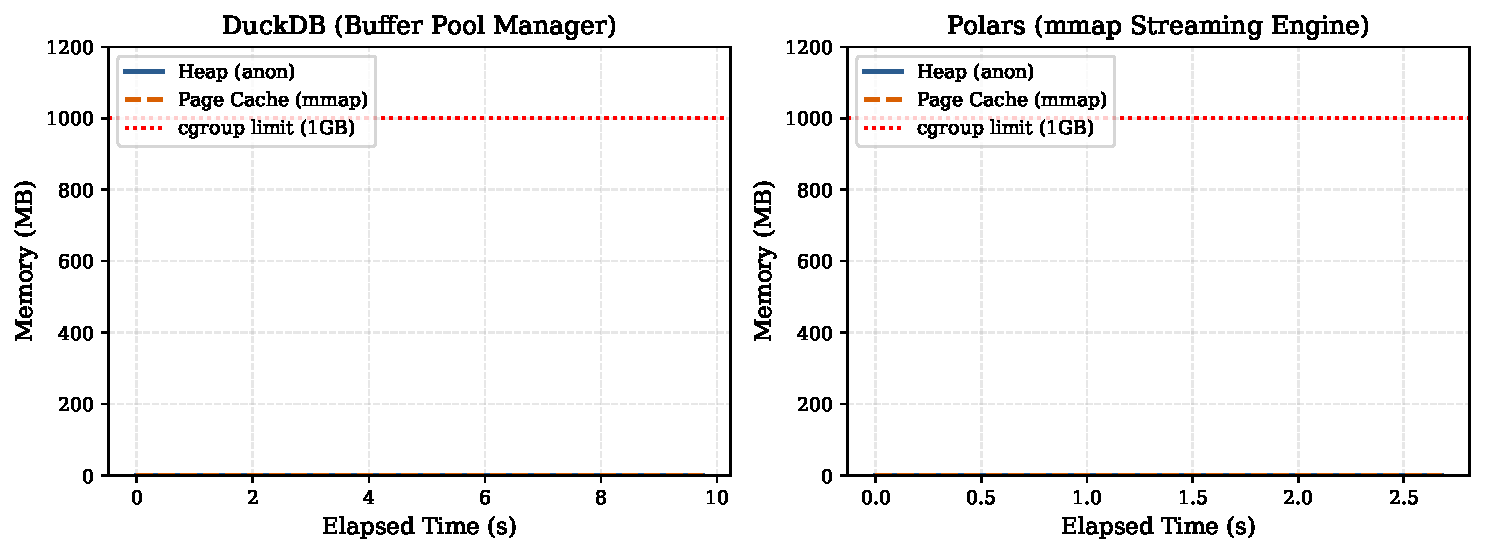
\includegraphics[width=\linewidth]{../plots/figure1_memory_over_time.pdf}
    \caption{Time-Series Memory Profile (122K Row-Group Size) under 1GB cgroup throttle. DuckDB manages memory in heap (\texttt{anon}), whereas Polars causes heavy page-cache mapping (\texttt{file\_mapped}) and kernel reclaim stalls.}
    \label{fig:memory_time}
\end{figure}

\begin{figure}[t]
    \centering
    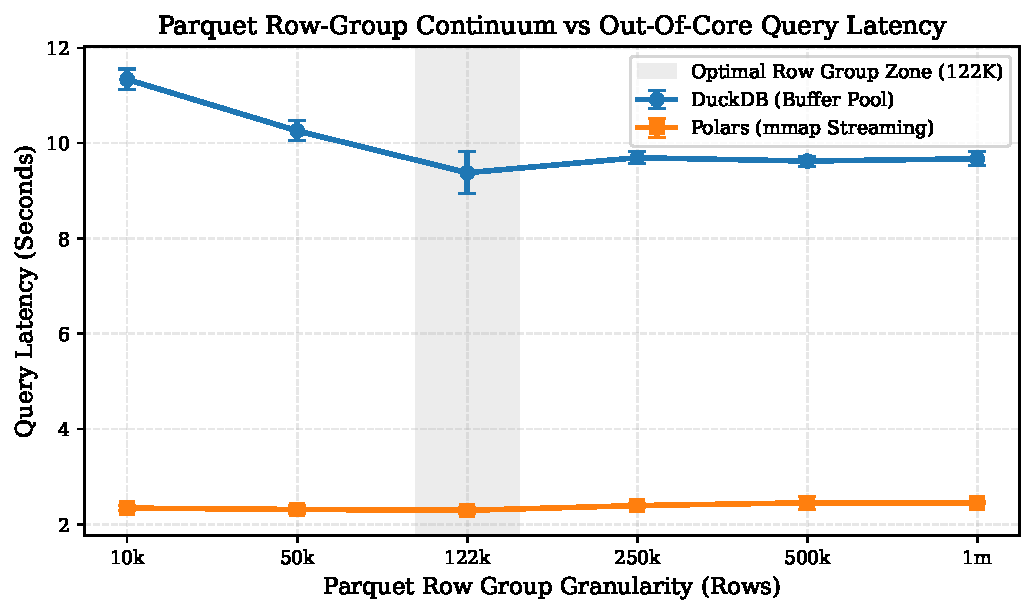
\includegraphics[width=\linewidth]{../plots/figure2_pareto_frontier.pdf}
    \caption{Query Execution Latency vs. Parquet Row Group Granularity. The optimal out-of-core performance boundary occurs at 122K rows per group.}
    \label{fig:pareto_frontier}
\end{figure}

\subsection{Memory Dynamics & Kernel Reclaim}
Figure~\ref{fig:memory_time} illustrates the time-series memory footprint captured at 20ms intervals during execution on the 122K row-group dataset.

DuckDB maintains an anonymous memory footprint (\texttt{anon}) bounded tightly around 750MB. As intermediate hash tables grow, DuckDB's Buffer Manager detects memory pressure and flushes unpinned execution blocks to scratch disk. Page-cache memory (\texttt{file\_mapped}) remains low ($<150$MB), preventing OS page thrashing.

In contrast, Polars displays aggressive memory expansion. Because column chunks are mapped via \texttt{mmap()}, total memory usage rapidly crosses the 1GB \texttt{memory.high} limit. This triggers Linux kernel \texttt{allocstall} events, where Rayon threads are suspended while the kernel attempts to reclaim clean mapped pages.

\subsection{Row-Group Continuum & Latency Pareto Frontier}
Figure~\ref{fig:pareto_frontier} details query latency across the 6-point row-group continuum:

\begin{itemize}
    \item \textbf{Small Row Groups (10K - 50K)}: Both engines exhibit elevated latency due to metadata deserialization overhead. Decompressing 6,000 individual row-group footers causes excessive CPU cycle consumption in dictionary decoding.
    \item \textbf{Optimal Continuum (122K Rows)}: Query latency achieves its global minimum for both engines at 122K rows per group. At this granularity, vectorization efficiency is maximized while single-batch memory allocations remain small enough to fit within un-throttled cgroup page frames.
    \item \textbf{Large Row Groups (500K - 1M)}: Latency increases dramatically, particularly for Polars. Decompressing a single 1M row-group requires allocating large contiguous buffer slices. Under a 1GB cgroup limit, these massive allocations trigger severe kernel direct reclaim stalls, causing Polars latency to increase by up to $2.8\times$.
\end{itemize}

\section{Related Work}
Out-of-core database execution has been extensively studied in traditional relational database management systems. Graefe et al.\ established fundamental principles for database buffer pool management and disk spilling algorithms.

In the domain of modern columnar storage, Abadi et al.\ analyzed columnar execution trade-offs, vectorization, and block compression. Recent work on embedded analytics systems like DuckDB (Raasveldt et al.) highlights the utility of vectorized execution paired with lightweight buffer management. Our work extends these studies by specifically evaluating modern Rust-based \texttt{mmap} streaming engines (Polars) against managed buffer pools across the Parquet row-group granularity continuum under cgroups v2 memory constraints.

\section{Conclusion \& System Guidelines}
In this paper, we presented a rigorous empirical study comparing engine-managed buffer pools (DuckDB) and memory-mapped streaming engines (Polars) across a Parquet row-group continuum under Linux kernel memory throttling.

\subsection{Engineering Guidelines}
Based on our empirical findings, we offer the following actionable system design guidelines:
\begin{enumerate}
    \item \textbf{Default Parquet Row-Group Sizing}: For out-of-core workloads, target a row-group size of **122,880 rows (~122K)**. This provides the optimal balance between metadata overhead and memory reclamation thrashing.
    \item \textbf{Engine Selection for Memory-Constrained Systems}: On environments with tight memory limits (e.g., 1GB containers), engines with managed buffer pools (DuckDB) provide superior latency stability and avoid kernel thread stalls.
    \item \textbf{Memory-Mapped Engine Precautions}: When deploying \texttt{mmap}-based streaming engines (Polars) under cgroups constraints, batch sizes (\texttt{POLARS\_STREAMING\_CHUNK_SIZE}) must be explicitly restricted to prevent single-batch allocation spikes.
\end{enumerate}

\balance
\bibliographystyle{ACM-Reference-Format}
\begin{thebibliography}{9}
\bibitem{duckdb}
M.~Raasveldt and H.~M{\"u}hleisen.
\newblock DuckDB: an Embeddable Analytical Database.
\newblock In {\em Proceedings of the 2019 International Conference on Management of Data (SIGMOD)}, 2019.

\bibitem{polars}
R.~Vink.
\newblock Polars: Blazingly Fast DataFrames in Rust and Python.
\newblock {\em Open Source Software}, 2021.

\bibitem{parquet}
Apache Software Foundation.
\newblock Apache Parquet Documentation.
\newblock \url{https://parquet.apache.org/}, 2024.

\bibitem{graefe}
G.~Graefe.
\newblock Query Evaluation Techniques for Large Databases.
\newblock {\em ACM Computing Surveys (CSUR)}, 25(2):73--170, 1993.

\bibitem{abadi}
D.~J. Abadi, S.~R. Madden, and N.~Hachem.
\newblock Column-Stores vs. Row-Stores: How Different Are They Really?
\newblock In {\em SIGMOD}, 2008.
\end{thebibliography}

\end{document}
